% Setup - do not change
\documentclass[11pt]{article}
\usepackage[top=0.9in, left=0.9in, bottom=0.9in, right=0.9in]{geometry} 
\usepackage{parskip}

\usepackage[english]{babel}
\usepackage[utf8]{inputenc}
\usepackage{amsmath,amsthm,amssymb,graphicx,pdfpages,lipsum,hyperref}
\usepackage[none]{hyphenat}
\usepackage{csquotes}

\setlength\parindent{0pt}
%%%%%%%%%%%%%%%%%%%%%%%%%%%%%%%%%%%%%%%%%%%%%%%%%%%%%%%%%%%%%%%%%%%
% add other packages here if required

%% Bibliography are specified in this file. You can also choose inline bib style if you want to. But make sure your citation style is consistent (and proper)
% For more details on citation: https://library.unimelb.edu.au/recite
\usepackage[sorting = none]{biblatex}
\addbibresource{references.bib}

%%%%%%%%%%%%%%%%%%%%%%%%%%%%%%%%%%%%%%%%%%%%%%%%%%%%%%%%%%%%%%%%%%% the '%' symbol denotes comments

% Begin document creation
% DELETE THE \lipsum PLACEHOLDERS WHEN YOU BEGIN
\title{\textbf{New York Taxi Trip Tip Analysis and Predict }}
\author{
Junbo Hu \\
Student ID: 1038361 \\
%% Replace the link with your github repo
% 1. Remember to escape underscore (\_) in the link.
% 2. Remember to include the commit you want to submit in the link
\href{https://github.com/MAST30034-Applied-Data-Science/mast30034-project-1-jumbo11111}{Github repo with commit}
}

\begin{document}
\maketitle

\section{Introduction}
% Link to a 30 min tutorial if you require revision: https://www.overleaf.com/learn/latex/Learn_LaTeX_in_30_minutes


Gig economy is becoming more and more popular in recent years, and it has become one of income for many people in United States. Besides, there is a culture of tipping throughout the United States, while the tip is an important part of income for service industry practitioners. Taxi drivers especially Lyft or Uber drivers is groups of people who benefit from gig economy, and tip from passenger contributes a lot to their income. For drivers, estimating tip income accurately is important for planning works. With the development and application of big data technology, more and more companies, and organizations such as Uber, Lyft and the Taxi and Limousine Commission (TLC) would like to share the trip data to public, these data typically include essential data related to a trip, among them contains the amount of tip.\cite{ref1}.

In this work, we selected Yellow Taxi Trip Data from NYC and the objective of this work is analyzing which factors will influence the tip for driver in a trip and finding a model that can predict the amount of tip for a trip. It might be beneficial for drivers and help them works more efficiently and it also might help platforms like Uber design better algorithm to improve drivers’income.


% You can have \section{}, \subsection{}, and \subsubsection{}
\section{Preprocessing, Analysis, and Geospatial Visualisation}
\subsection{Dataset}
\begin{enumerate} 
    \item Yellow Taxi Trip Data
    
The data is provided by New York city government, it includes fields capturing pick-up and drop-off dates/times, pick-up and drop-off locations, trip distances, itemized fares, rate types, payment types, and driver-reported passenger counts. This work picks the data from September to December in 2021. The data downloaded is in Apache Parquet format, which can be loaded by pandas package directly. It also includes taxi zoon maps to reference.\cite{ref2}.

    \item Weather Data
    
The weather data is from Visual Crossing, a website provides weather history data around the world and allows user to query data by different conditions. It includes the average, maximum, minimum temperature for a day, wind speed, visibility, humidity, and other weather attributes. This work picks the hourly data in New York from September to December in 2021, and data downloaded is in csv format.

\end{enumerate}

\subsection{Pre-process}
\begin{enumerate}
    \item Data Cleaning

After calculating the share of empty data in the dataset, the result shows that it is reasonable to delete all empty data because the share of them is low which may not influence the whole dataset. Another step took to clean the data is dropping outliers with the help of box plot. In the taxi trip data, fare amount, tip amount and total amount are variables which contains lots of outliers. In this work, the outliers are removed with the help of interquartile range. The results of this process are showed in Figure 1 and Figure 2.

\begin{figure}[h]
\centering
\begin{minipage}[t]{0.48\textwidth}
\centering
    \includegraphics[width=0.75\textwidth]{plots/amount-before-clean.png}
    \caption{Outliers of amounts before cleaning}
\end{minipage}
\begin{minipage}[t]{0.48\textwidth}
\centering
    \includegraphics[width=0.75\textwidth]{plots/amount-after-clean.png}
    \caption{Outliers of amounts after cleaning}
\end{minipage}
\end{figure}

Finally, data which may not helpful for this work is removed by following conditions:
\begin{itemize} 
    \item Records whose passenger count or trip distance is 0.
    \item Records whose pick-up or drop-off data time is out of range.
    \item Records whose fare amount is pretty low (less than 2.5 dollars).
\end{itemize} 

Weather history data query from database has already been examined by website owner so that there is no empty value for important attributes such as temperature, visibility. Bases on this opinion, data cleaning is not applied on weather data.

    \item Feature Engineering
    
To better research the influence of datetime, this work adds these features: day, week, month, weekday, starting hours, ending hours. In addition, the trip time calculated by timestamp of picking and dropping is also added.

For weather data, some features may be helpful are picked: feels like temperature, humidity, windspeed, visibility and conditions. Because conditions attribute is category label, one-hot encoding is applied on it.

The processed taxi data and weather data are combined in a new dataset. The weather data for a trip is based on hour of pick-up time.
    
\end{enumerate}



\subsection{Aalysis and Visualisation}

To better understand how features interact, correlation matrix is computed for the dataset, and it is represented in a heat map (Figure 3-4). The heat maps illustrate that tip could be significantly influenced by trip distance, trip time and total fare, besides, weather also influence it in some degree.


\begin{figure}[h]
\centering
\begin{minipage}[t]{0.48\textwidth}
\centering
    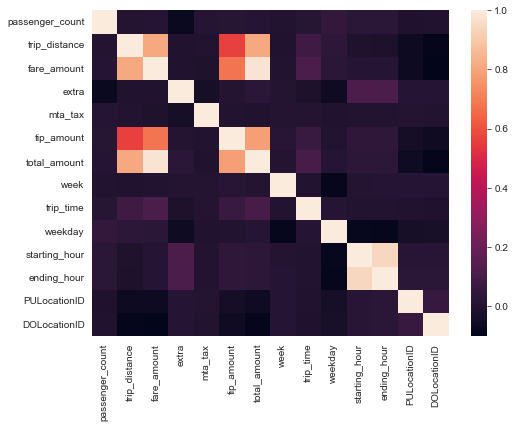
\includegraphics[width=0.75\textwidth]{plots/heatmap1.png}
    \caption{Heat map for taxi trip data}
\end{minipage}
\begin{minipage}[t]{0.48\textwidth}
\centering
    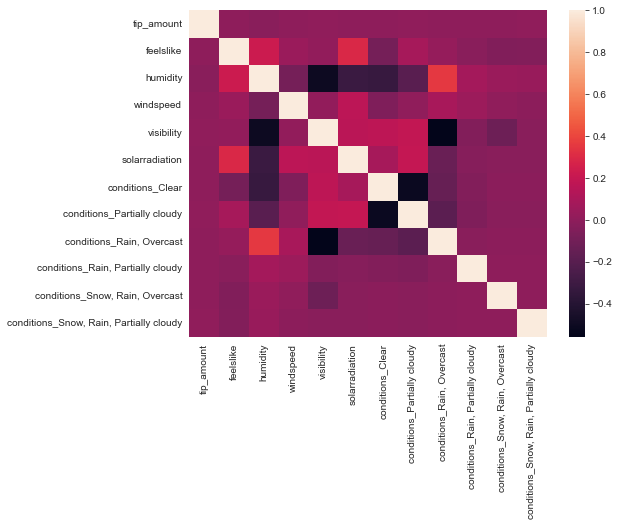
\includegraphics[width=0.75\textwidth]{plots/heatmap2.png}
    \caption{Heat map for weather data}
\end{minipage}
\end{figure}


In the next step, the distributions of features are visualized using histogram plot. Log transformation is applied on the data (Figure 5-6). Besides, this work also analysis the average tip for a trip in different weather conditions in Figure 7. In the period selected in this work, the temperature in New York is mainly in 0 to 30 Celsius degrees, the wind speed is slower than 30 meters/s and visibility is mainly higher that 10 kilometers. 
\begin{figure}[h]
\centering
\begin{minipage}[t]{0.48\textwidth}
\centering
    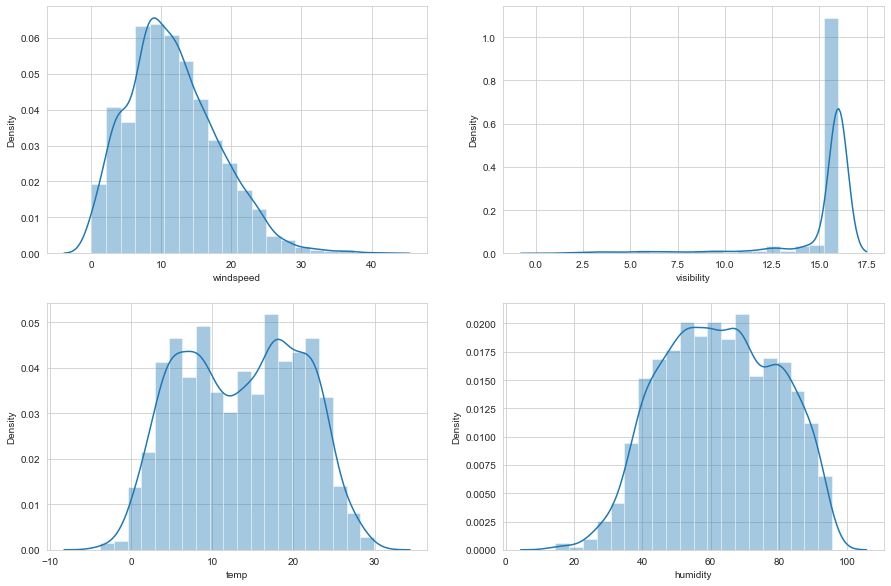
\includegraphics[width=0.75\textwidth]{plots/weather-1.png}
    \caption{Weather features distribution}
\end{minipage}
\begin{minipage}[t]{0.48\textwidth}
\centering
    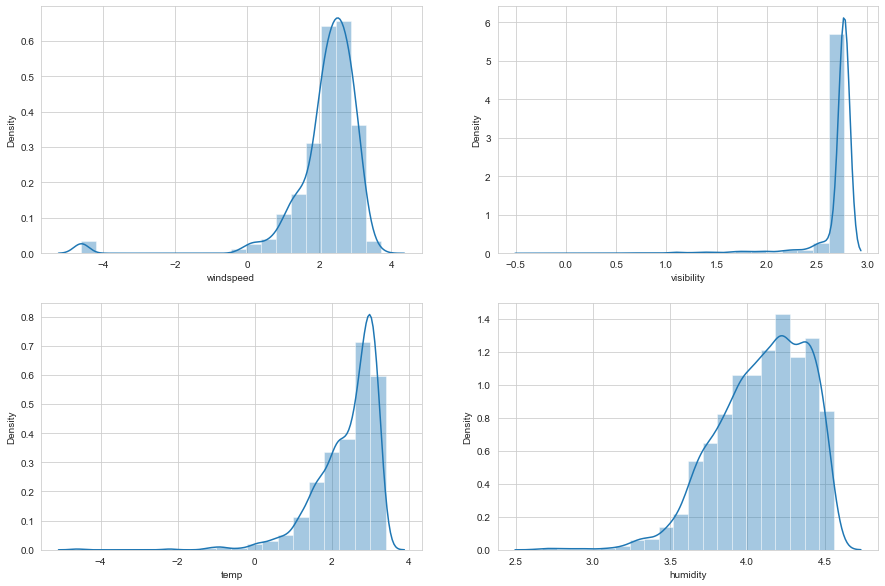
\includegraphics[width=0.75\textwidth]{plots/weather-2.png}
    \caption{Weather features distribution(With log transformation)}
\end{minipage}
\begin{minipage}[t]{0.35\textwidth}
\centering
    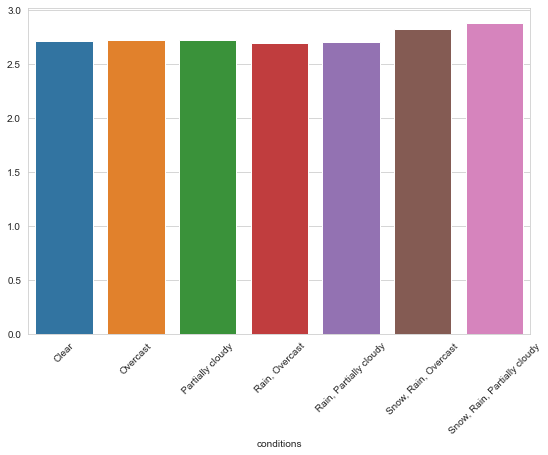
\includegraphics[width=0.75\textwidth]{plots/avg-tip-weather.png}
    \caption{Average tip by weather conditions}
\end{minipage}
\end{figure}

Figure 7 shows that for special weather conditions with rain or snow, the average tip is appreciably higher than other conditions.

As geographic-related data is provided, in this work, average drop-off, average tip and average fare are visualized in different destination region in a map graph. Most passengers pay the tip at the destination so that this work mainly analysis the effects of destination on tip. As the Figure 8-10 represent, high average fare and high average tip may happen in the same region, but both may not associate with average drop-off.


For region includes airport such as JFK and Newark, it could have both high fare and high tip. A surprise finding is that in rich region such as Manhattan, the average tip is not really high, although it is the highest drop-off region.


\begin{figure}[h]
\centering
\begin{minipage}[t]{0.48\textwidth}
\leftin
    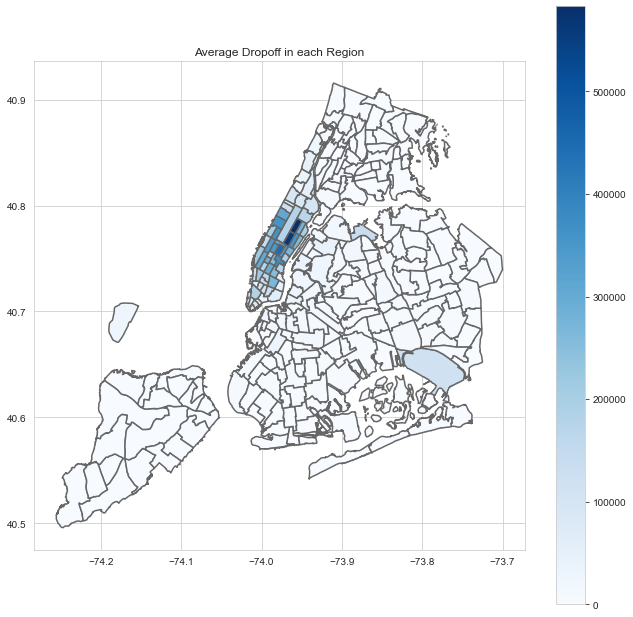
\includegraphics[width=0.75\textwidth]{plots/map1.png}
    \caption{Average drop-off by regions}
\end{minipage}
\begin{minipage}[t]{0.48\textwidth}
\centering
    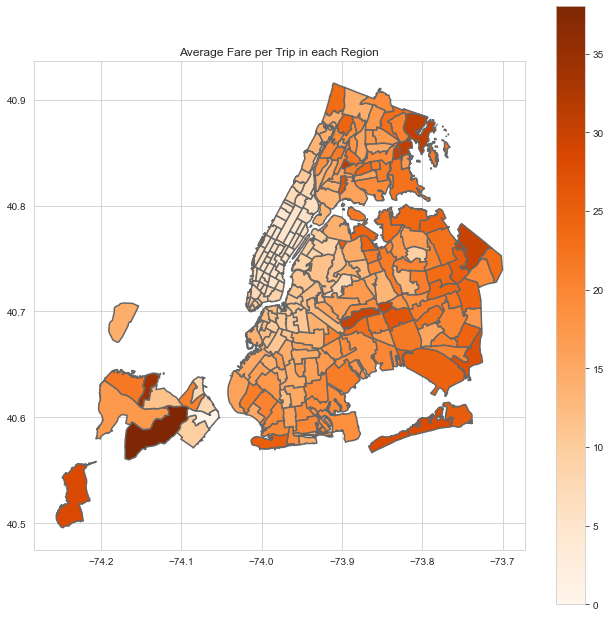
\includegraphics[width=0.75\textwidth]{plots/map2.png}
    \caption{Average fare by regions}
\end{minipage}
\begin{minipage}[t]{0.48\textwidth}
\centering
    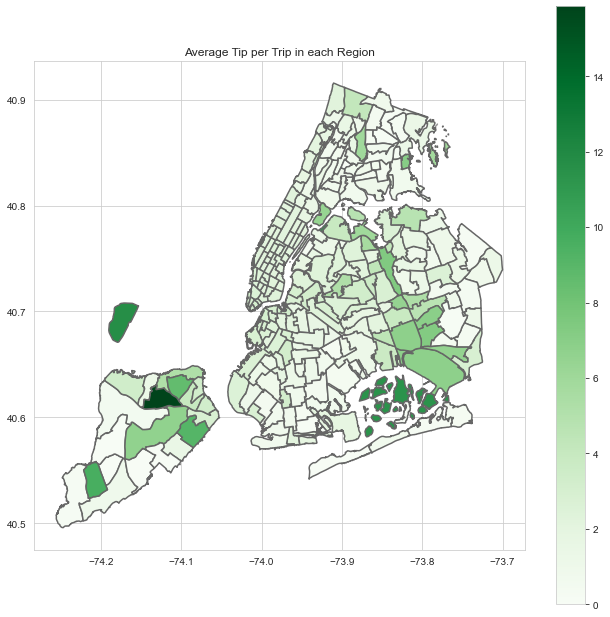
\includegraphics[width=0.75\textwidth]{plots/map3.png}
    \caption{Average tip by regions}
\end{minipage}
\end{figure}


By inspecting the relationship between the time of a day or day of a week and the trip frequency, trips occur more frequently around 12:00 to 18:00 in the afternoon between Tuesday to Friday. This work finds that the average tip in work days is a little higher then weekends, but there is no significant difference in different days of week. Furthermore, the results shows that passengers may pay more tip in the nigh, especially in period from 22:00 to 01:00 and from 04:00 to 05:00.

\section{Modelling}

Regression methods are used to building a model which can predict the tips for each trip. Linear regression and XGBoost regression are tested in this work. Before training the model, features:

'tip\_{}amount','total\_{}amount','tpep\_{}pickup\_{}datetime','tpep\_{}dropoff\_{}datetime','VendorID','RatecodeID', 

'conditions','store\_{}and\_{}fwd\_{}flag' and 'payment\_{}type' are removed from dataset. 

The whole data are spited into training set and test set. The size of training set is 70 percent of the origin data. To eliminate the influence of different range for features, min-max scale are applied on the data.

Linear regression analysis is widely used in data science which predicts the value of a variable based on the values of another variables. The variable to be predicted is called the dependent variable while variables used to predict the other variable's value is called the independent variable.\cite{ref4}

As this algorithm describe the relationship between independent variables and dependent variable using linear equation, it estimates the coefficients of such an equation. Linear regression fits a straight line or surface that minimizes the discrepancies between predicted and actual output values. Simple linear regression calculators that use a least squares method to discover the best-fit line for a set of paired data.

\begin{align}
    y_{i}=\beta _{0}+\beta _{1}x_{i}+\epsilon _{i}
\end{align}

\begin{align}
    MSE=\frac{1}{n}\sum_{i=1}^{n}(y_{i}-\hat{y}_{i} )^{2} 
\end{align}

XGBoost is an optimized distributed gradient boosting library designed to be highly efficient, flexible and portable. It implements machine learning algorithms under the Gradient Boosting framework.\cite{ref3}

To evaluate the performance of models, we calculated the score and MSE using API in scikit-learn. And this work takes sample of predicted values and real values, plots them in the same graph for comparison. The blue line is real value while the yellow line is predicted value. It is clearly that both models can predict accurate value, but for condition that there is no tip, they may give error predictions.

\begin{figure}[h]
\centering
\begin{minipage}[t]{0.48\textwidth}
\centering
    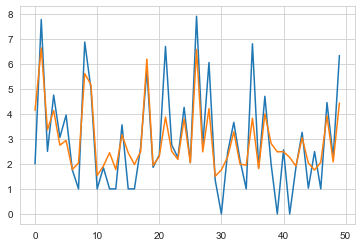
\includegraphics[width=0.75\textwidth]{plots/lr.png}
    \caption{Linear regression model}
\end{minipage}
\begin{minipage}[t]{0.48\textwidth}
\centering
    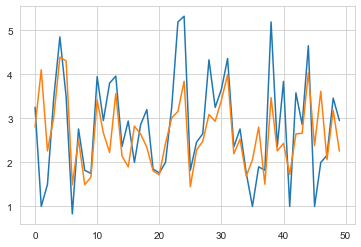
\includegraphics[width=0.75\textwidth]{plots/xgboost.png}
    \caption{XGBoost regression model}
\end{minipage}
\end{figure}

The following table shows details about performance in two models. They both have analogous performance and XGBoost model is a little bit better.

\begin{center}
\begin{tabular}{||c c c c||} 
 \hline
 Model & Score-Train set & Score-Test set & MSE \\ [0.5ex] 
 \hline\hline
 Linear Regression & 0.4736 & 0.4736 & 1.177 \\ 
 \hline
 XGBoost Regression & 0.5107 & 0.5061 & 1.10 \\
 \hline
\end{tabular}
\end{center}

In this work, the sum of predicted value in test set is also calculated, and it is compared with real value. The real sum is 7167450, the sum by Linear Regression model is 7166491 and for XGBoost it is 7166592.

\section{Recommendations}

In this work, only data in four months are used to research, long tern data could help to improve the accuracy. For external data, only weather is considered. Moreover, some other external data set such as the traffic conditions, oil price can be also considered in this kind of work.

Regression model may have tiny error when predicting tip for a single trip, however, as there are enough records in a big sample, the sum of predicted values in close to the real value. In further, for a single trip, it may be helpful if using classifier to implements classification on whether passenger will pay tip or the level of tip such as tiny, general, much.

Furthermore, only two regression models is tested in this work, other regression algorithms such as SVR (Support Vector Machine Regression), Logistic Regression and neural network could be considered.


\section{Conclusion}

In conclusion, there are many factors which may influence tip in a trip, and it is predictable. Visualization plays an important role in data analysis in this work. It is meaningful to company like Uber in designing an algorithm which helps to schedule drivers efficiently and improve their tip income. 



\clearpage

% BEGIN REFERENCES SECTION
\printbibliography

\end{document}